\section{Experiments}\label{sec:experiments}\label{sec:results}

This section evaluates TE-Q-Transformer under a fixed NASA protocol and then tests whether the learned behaviour transfers beyond that protocol. Section~\ref{sec:experiment_setup} states the data, split, training settings, and comparison models. Section~\ref{sec:nasa_case} reports the primary NASA case study. Section~\ref{sec:contemporary_comparison} places the proposed model among recurrent, convolutional, linear, attention-based, and quantum-recurrent alternatives. Section~\ref{sec:ablation} isolates the contribution of physics-guided temperature encoding, temperature-dependent mechanisms, the quantum representation, and architectural components. Section~\ref{sec:generalization} examines cross-cell and temporal generalization together with run-to-run variability. Section~\ref{sec:calce} reports a final zero-shot test on the independent CALCE dataset. The NASA temperatures used at test time also appear in the training pool, so the study does not claim unseen-temperature generalization.

\subsection{Experimental Setup}
\label{sec:experiment_setup}

\subsubsection{Dataset and Preprocessing}
\label{sec:data_preprocess}

Two public laboratory datasets are used. NASA PCoE 18650 cells~\cite{saha2007battery} form the primary benchmark. CALCE CS2 cells~\citep{w9rg-7173-25} are reserved for external validation and are never used to fit a scaler, select a model, or update weights.

NASA inputs are cycle-level discharge records with four channels: voltage, current, temperature in degrees Celsius, and intra-cycle normalized time. Each cycle is linearly resampled to a sequence of length $L=512$. State of health is defined per cell as
\begin{equation}
\mathrm{SOH}_k = C_k / C_0,
\end{equation}
where $C_k$ is the measured capacity of cycle $k$ and $C_0$ is the first-cycle capacity of the same cell. Voltage, current, and normalized time are scaled with a min--max scaler fitted on the NASA training partition only. Temperature is left in raw Celsius so that the Arrhenius mapping receives physically meaningful values. CALCE windows use the same four-channel layout and the frozen NASA scaler. Because the archived CS2 files do not provide a thermocouple channel, CALCE temperature is filled with a constant ambient value of $23\,^\circ$C.

Table~\ref{tab:data_stats} summarizes dataset size and preprocessing. Table~\ref{tab:exp_split} defines evaluation roles and is not repeated here.

\begin{table*}[htbp]
\centering
\footnotesize
\caption{Dataset statistics and preprocessing used in this study. Evaluation roles are defined in Table~\ref{tab:exp_split}.}\label{tab:data_stats}
\begin{tabular*}{\textwidth}{@{}LLLL@{}}
\toprule
Item & NASA & CALCE \\
\midrule
Cells used & B0005--B0007, B0029--B0032, B0018, B0053 & CS2\_35--CS2\_38 \\
Cycles / windows & 660 training + 187 test cycles & 3909 test windows \\
Channels & $V$, $I$, $T$, $t_{\mathrm{norm}}$ & same four channels \\
Window length & 512 & 512 \\
Resampling & linear to 512 samples per cycle & archived cycle windows \\
Scaling & train-only min--max on $V$, $I$, $t_{\mathrm{norm}}$ & frozen NASA scaler \\
Temperature & raw $^\circ$C & constant $23\,^\circ$C fill \\
SOH & $C_k/C_0$ & $C_k/C_0$ \\
Role & primary benchmark & zero-shot external test \\
\bottomrule
\end{tabular*}
\end{table*}

\subsubsection{Evaluation Protocol}
\label{sec:evaluation_protocol}

All NASA experiments use one hybrid cell-level split (Table~\ref{tab:exp_split}). Training uses B0005, B0006, B0007, B0029, B0030, B0031, and B0053 cycles 0--36 ($N=660$). Testing uses B0018 ($n=132$), B0032 ($n=39$), and B0053 cycles 37--52 ($n=16$). B0018 and B0032 are unseen cells. B0053 cycles 37--52 are a temporal holdout on a cell that already contributed early cycles to training; B0053 is not an unseen cell. Nominal ($24\,^\circ$C), elevated ($43\,^\circ$C), and sub-ambient ($4\,^\circ$C) temperatures all appear in training. The protocol therefore tests cross-cell generalization and short temporal extrapolation, not temperature hold-out.

Cells and cycles are partitioned before windowing. There is no independent test-cell normalization, no test-based hyperparameter search, no test-based model selection, and no test-set calibration. Reported NASA overall RMSE, MAE, MAPE, and $R^2$ are unweighted means of the three evaluation settings unless a table states otherwise.

CALCE CS2\_35--CS2\_38 are used only as zero-shot external cells. No CALCE cell enters training, scaler fitting, or model selection. The constant $23\,^\circ$C fill means that CALCE cannot support a temperature-generalization claim.

\begin{table*}[htbp]
\centering
\footnotesize
\caption{Train--test assignment used throughout the NASA study, together with the CALCE zero-shot test. B0053 is a temporal holdout, not an unseen cell.}\label{tab:exp_split}
\begin{tabular*}{\textwidth}{@{}LLLL@{}}
\toprule
Dataset & Partition & Cells / cycles & Role \\
\midrule
NASA & Train & B0005, B0006, B0007, B0029, B0030, B0031, B0053 0--36 & Seen cells + early B0053 \\
NASA & Test & B0018 & Unseen cell, $24\,^\circ$C \\
NASA & Test & B0032 & Unseen cell, $43\,^\circ$C \\
NASA & Test & B0053 37--52 & Temporal extrapolation, $4\,^\circ$C \\
CALCE & Test only & CS2\_35, CS2\_36, CS2\_37, CS2\_38 & Zero-shot external cells, $23\,^\circ$C \\
\bottomrule
\end{tabular*}
\end{table*}

\subsubsection{Implementation Details}
\label{sec:implementation_details}

Common training settings are listed in Table~\ref{tab:exp_settings}. Each input is a length-512 window. Optimization uses AdamW with learning rate $10^{-3}$, batch size 8, a maximum of 80 epochs, and gradient-norm clipping at $1.0$. The learning-rate scheduler is ReduceLROnPlateau (factor $0.5$, patience 10). Early stopping uses training MSE with patience 20. No independent validation split was used in the reported runs; the retained model is the lowest training-loss epoch. This is a protocol limitation and is stated as such.

The quantum circuit uses four qubits and is executed as a PennyLane \mbox{\texttt{default.qubit}} state-vector simulation. It is not physical quantum hardware. Evaluation metrics are RMSE, MAE, MAPE (\%), $R^2$, and maximum absolute error (MaxE). The main NASA experiments use seed 42. Run-to-run variability is later assessed on the predefined seeds 42--46. Weight decay is $5\times10^{-2}$ in the validated reference configuration and $1\times10^{-2}$ in the independent retraining used for generalization and multi-seed analysis. Those two TE-Q-Transformer result contexts are retained separately and are not merged.

\begin{table*}[htbp]
\centering
\footnotesize
\caption{Common experimental settings for the NASA runs reported in this section.}\label{tab:exp_settings}
\begin{tabular*}{\textwidth}{@{}LL@{}}
\toprule
Item & Setting \\
\midrule
Input features & Voltage, current, temperature ($^\circ$C), intra-cycle time \\
Sequence length & 512 \\
SOH target & $C_k/C_0$ (per cell) \\
Loss & Training MSE \\
Optimizer & AdamW; learning rate $10^{-3}$ \\
Batch size / max epochs & 8 / 80 \\
Scheduler & ReduceLROnPlateau (factor 0.5, patience 10) \\
Early stopping & Patience 20 on training loss (no validation split) \\
Gradient clipping & Maximum norm $1.0$ \\
Weight decay (reference configuration) & $5\times10^{-2}$ \\
Weight decay (independent retraining) & $1\times10^{-2}$ \\
Quantum execution & PennyLane \mbox{\texttt{default.qubit}}, 4 qubits \\
Random seeds & 42 (main NASA runs); 42--46 (multi-seed study) \\
Hardware record & CPU simulator for the matched classical/quantum comparison; CUDA for independent retraining \\
\bottomrule
\end{tabular*}
\end{table*}

\subsubsection{Comparison Methods}
\label{sec:baseline_comparison}

The scored comparison comprises eight classical sequence models, two hybrid quantum-recurrent models, and the proposed TE-Q-Transformer (Table~\ref{tab:exp_baselines}). The baselines cover recurrent encoders (LSTM, GRU), convolutional and temporal models (CNN1D, TCN), a linear decomposition model (DLinear), attention-based models (Transformer, PatchTST, iTransformer), and quantum-recurrent models (QLSTM, QNN-GRU)~\citep{wang2024state,zhang2023accurate,giuliano2025transformer,soon2025hybrid,wang2026prediction}. All scored models use the same NASA split, window length, and train-only scaler.

TimesNet was implemented under the same interface but is excluded from the scored comparison because of disproportionate computational cost at $L=512$ (approximately $14.3$ million parameters and about one hour per CPU epoch). A gate-level QGRU was also implemented; a completed scored NASA run is not available, so no QGRU test number is reported.

In the main benchmark, the ten baselines are trained from scratch under the common protocol, while TE-Q-Transformer is held at the validated reference configuration. An independent retraining of five designated models is used later for trajectory-level generalization and multi-seed analysis.

\begin{table*}[htbp]
\centering
\footnotesize
\caption{Comparison methods used in the scored NASA benchmark. Parameter counts are trainable parameters under the shared NASA interface. TimesNet is excluded because of disproportionate cost.}\label{tab:exp_baselines}
\begin{tabular*}{\textwidth}{@{}LLLLL@{}}
\toprule
Model & Family & Core architecture & Params & Quantum \\
\midrule
LSTM & Recurrent & LSTM encoder & 71\,105 & --- \\
GRU & Recurrent & GRU encoder & 54\,465 & --- \\
CNN1D & Convolutional & Conv1d stack & 47\,041 & --- \\
TCN & Convolutional & causal dilated TCN & 91\,841 & --- \\
DLinear & Linear & decomposition linear & 1\,031 & --- \\
Transformer & Attention & encoder attention & 80\,257 & --- \\
PatchTST & Attention & patch + channel independence & 109\,962 & --- \\
iTransformer & Attention & inverted tokens & 137\,473 & --- \\
QLSTM & Quantum-recurrent & quantum LSTM cell & 37\,853 & simulator \\
QNN-GRU & Quantum-recurrent & QNN + GRU & 29\,533 & simulator \\
TE-Q-Transformer & Proposed & physics-guided VQC + Transformer & 92\,554 & 4-qubit sim. \\
\bottomrule
\end{tabular*}
\end{table*}

\subsection{Case Study on the NASA Battery Dataset}
\label{sec:nasa_case}

\subsubsection{Dataset Description}
\label{sec:nasa_description}

The NASA Ames PCoE lithium-ion ageing set is the primary benchmark because it provides cycle-level voltage, current, and thermocouple records for commercial 18650 cells across more than one ambient temperature~\cite{saha2007battery}. The cells used here occupy three temperature groups: $24\,^\circ$C (B0005--B0007, B0018), $43\,^\circ$C (B0029--B0032), and $4\,^\circ$C (B0053). Figure~\ref{fig:nasa_setup} shows cycle counts by cell, temperature, and evaluation role. Training cells are available at all three temperatures, which is why a strong NASA test score cannot be read as evidence of unseen-temperature generalization.

\begin{figure}[htbp]
\centering
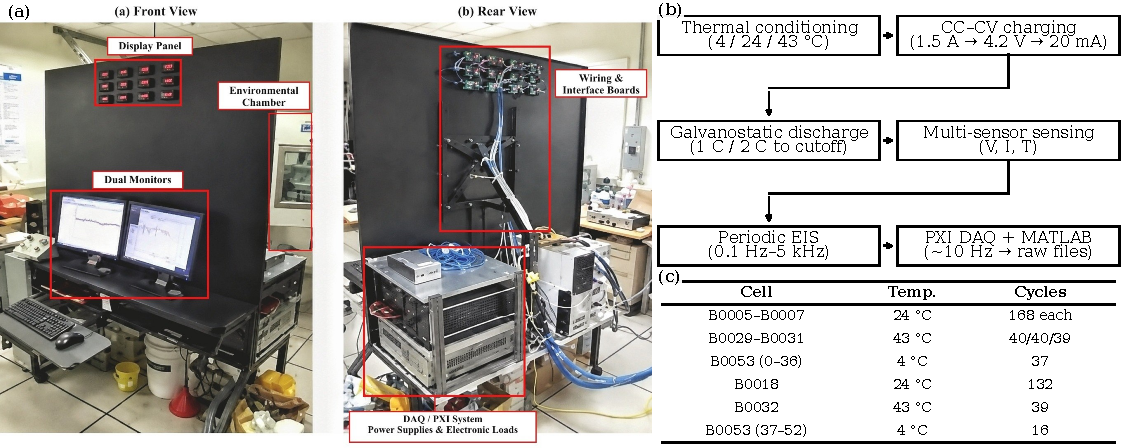
\includegraphics[width=\linewidth]{figs/fig2_nasa_experimental_setup.pdf}
\caption{NASA cells used in this study. Bar height is the number of discharge cycles. Labels above the bars give the ambient temperature. Colour indicates evaluation role: training, unseen-cell test, or temporal holdout on B0053.}
\label{fig:nasa_setup}
\end{figure}

\subsubsection{Evaluation Task Setup}
\label{sec:nasa_task_setup}

The NASA case study answers two complementary questions under the split in Table~\ref{tab:exp_split} and Figure~\ref{fig:nasa_generalization}(a).

Task A is cross-cell generalization: a model trained on B0005--B0007, B0029--B0031, and early B0053 is asked to estimate SOH on fully unseen B0018 and B0032. Task B is temporal extrapolation: the same model is asked to continue B0053 after seeing only cycles 0--36. The two settings are not equivalent. B0053 is partially observed, and the held-out tail contains only 16 cycles. B0053 is therefore not an unseen cell, and the $4\,^\circ$C condition is not an unseen temperature.

\subsubsection{Overall Results}
\label{sec:nasa_results}

The validated TE-Q-Transformer configuration was first evaluated under this fixed NASA protocol (seed 42, weight decay $5\times10^{-2}$). Table~\ref{tab:e01_ref} reports the cell-wise and macro metrics that serve as the proposed-model reference for the remainder of the NASA benchmark.

Macro RMSE is $0.0168$, MAE $0.0141$, MAPE $1.56\%$, and $R^2$ $0.870$. Error is not uniform across the three test settings. Unseen B0018 has the largest error (RMSE $0.0271$, MaxE $0.1022$). Unseen B0032 and the B0053 temporal tail are closer to the target (RMSE $0.0119$ and $0.0113$). The macro MaxE of $0.1022$ is the true maximum absolute error over all $187$ test cycles and occurs on B0018; it is not the mean of the three cell-wise maxima.

These numbers indicate that the reference configuration can follow unseen-cell fade at $24\,^\circ$C and $43\,^\circ$C and can continue a short cold-temperature tail, while the remaining point-wise error is concentrated on B0018. They do not yet identify which design choices produce that behaviour, nor how the model ranks against contemporary alternatives. Those questions are taken up next. An independently retrained configuration, used later for trajectory and multi-seed analysis, is not substituted for Table~\ref{tab:e01_ref}.

\begin{table*}[htbp]
\centering
\footnotesize
\caption{Validated TE-Q-Transformer reference on the NASA test settings (seed 42). Macro MaxE is the maximum absolute error over all test cycles, not the mean of cell-wise MaxE.}\label{tab:e01_ref}
\begin{tabular*}{\textwidth}{@{}LCCCCC@{}}
\toprule
Setting & RMSE & MAE & MAPE & $R^2$ & MaxE \\
\midrule
B0018 (unseen) & 0.0271 & 0.0223 & 2.66 & 0.894 & 0.1022 \\
B0032 (unseen) & 0.0119 & 0.0105 & 1.03 & 0.902 & 0.0237 \\
B0053-test (temporal) & 0.0113 & 0.0095 & 0.99 & 0.814 & 0.0220 \\
Macro & 0.0168 & 0.0141 & 1.56 & 0.870 & 0.1022 \\
\bottomrule
\end{tabular*}
\end{table*}

\subsection{Comparison with Contemporary Methods}
\label{sec:contemporary_comparison}

\subsubsection{Overall Performance}
\label{sec:overall_benchmark}

The proposed model was compared with recurrent, convolutional, linear, attention-based, and quantum-recurrent baselines under the same NASA split and seed 42 (Figure~\ref{fig:main_performance}; Table~\ref{tab:main_benchmark}). Among the evaluated models, TE-Q-Transformer recorded the lowest macro RMSE, MAE, and MAPE and the highest macro $R^2$. QNN-GRU is the closest trained baseline on macro RMSE ($0.0304$). Attention models occupy the next RMSE tier ($0.034$--$0.039$) with mixed $R^2$. The ranking is not uniform at the cell level: CNN1D recorded a lower RMSE on unseen B0018 ($0.0255$ versus $0.0271$). The comparison uses a single seed and is not a statistical test.

TE-Q MaxE in Table~\ref{tab:main_benchmark} is the true maximum absolute error ($0.1022$ on B0018). Cell-wise values for the proposed model remain those in Table~\ref{tab:e01_ref}. Training time for the frozen reference is omitted because it is not comparable to the ten models trained from scratch in this benchmark.

\begin{table*}[htbp]
\centering
\footnotesize
\caption{NASA performance comparison under the fixed cross-cell protocol. Overall metrics are unweighted means of B0018, B0032, and B0053-test. TE-Q-Transformer is the validated reference configuration and is not retrained in this comparison. TimesNet and QGRU are not scored.}\label{tab:main_benchmark}
\begin{tabular*}{\textwidth}{@{}LCCCCCCC@{}}
\toprule
Model & RMSE~$\downarrow$ & MAE~$\downarrow$ & MAPE~$\downarrow$ & $R^2$~$\uparrow$ & MaxE~$\downarrow$ & Params & Train (s) \\
\midrule
LSTM & 0.0416 & 0.0367 & 4.07 & $-$0.076 & 0.0904 & 71\,105 & 24.5 \\
GRU & 0.0642 & 0.0565 & 6.22 & $-$1.680 & 0.1631 & 54\,465 & 22.3 \\
CNN1D & 0.0509 & 0.0457 & 4.78 & $-$3.191 & 0.1245 & 47\,041 & 25.1 \\
TCN & 0.0535 & 0.0452 & 5.09 & $-$0.341 & 0.1491 & 91\,841 & 34.0 \\
DLinear & 0.0624 & 0.0568 & 5.88 & $-$2.232 & 0.1853 & 1\,031 & 15.5 \\
Transformer & 0.0346 & 0.0287 & 3.14 & 0.218 & 0.1123 & 80\,257 & 61.6 \\
PatchTST & 0.0387 & 0.0333 & 3.69 & 0.321 & 0.1457 & 109\,962 & 63.1 \\
iTransformer & 0.0341 & 0.0298 & 3.28 & 0.533 & 0.1165 & 137\,473 & 58.7 \\
QLSTM & 0.0445 & 0.0386 & 4.35 & $-$0.336 & 0.1066 & 37\,853 & 282.3 \\
QNN-GRU & 0.0304 & 0.0248 & 2.61 & 0.258 & 0.0725 & 29\,533 & 284.8 \\
TE-Q-Transformer$^{\mathrm{a}}$ & \textbf{0.0168} & \textbf{0.0141} & \textbf{1.56} & \textbf{0.870} & 0.1022 & 92\,554 & --- \\
\bottomrule
\end{tabular*}
\vspace{2pt}
\begin{minipage}{\textwidth}
$^{\mathrm{a}}$Validated reference configuration. Its training time is not comparable to the ten models trained from scratch and is omitted.
\end{minipage}
\end{table*}

\begin{figure*}[htbp]
\centering
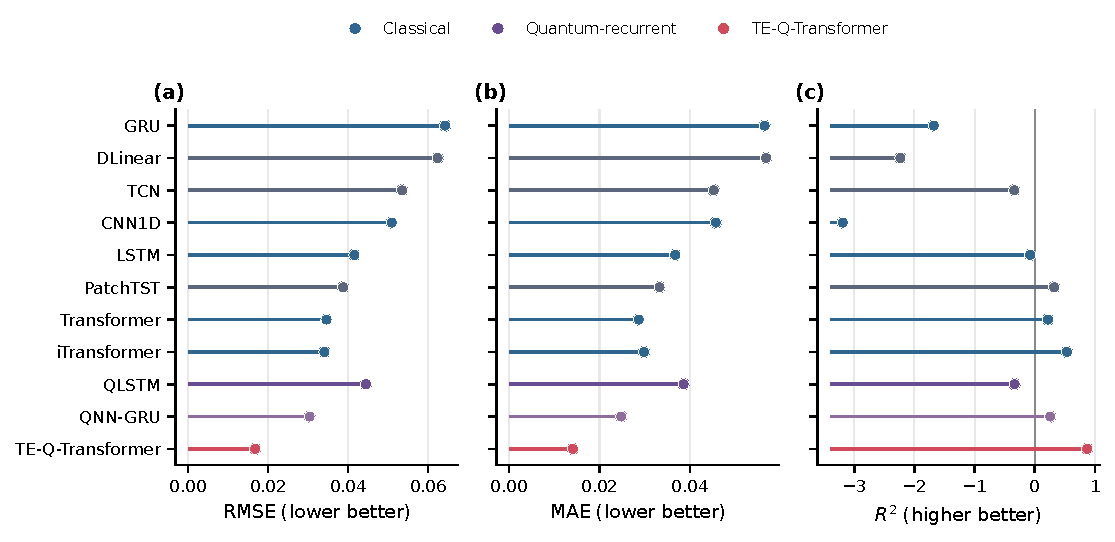
\includegraphics[width=\textwidth]{figs/fig6_main_performance.pdf}
\caption{Comparison of representative models under the fixed NASA cross-cell protocol. Models are grouped by family and ordered by RMSE within family. (a)~RMSE, (b)~MAE, (c)~$R^2$. TE-Q-Transformer is the validated reference configuration. Single seed 42.}
\label{fig:main_performance}
\end{figure*}

\subsubsection{Model-wise Analysis}
\label{sec:modelwise}

The family-level pattern in Figure~\ref{fig:main_performance} is more informative than the aggregate ranking alone. Recurrent models (LSTM, GRU) keep moderate RMSE on some cells but do not produce a stable positive macro $R^2$. Convolutional and linear models are weaker on the aggregate, and the failure is setting-specific rather than uniform: CNN1D collapses on the short B0053 tail ($R^2=-10.45$) even though it is competitive on B0018, while DLinear collapses on B0032 ($R^2=-7.16$). Attention models reduce RMSE relative to the recurrent group, yet $R^2$ remains mixed, which is consistent with a protocol that mixes a long unseen cell, a short unseen cell, and a 16-cycle temporal tail.

The two quantum-recurrent models diverge. QNN-GRU is the strongest trained baseline. QLSTM does not improve on LSTM. A quantum module by itself is therefore not a sufficient explanation of the proposed-model result. The contribution of the quantum representation under a matched downstream architecture is isolated in Section~\ref{sec:quantum_analysis}.

\subsubsection{Computational Analysis}
\label{sec:computational_analysis}

Table~\ref{tab:compute} and Figure~\ref{fig:compute} report parameter counts and recorded wall-clock times. TE-Q-Transformer has $92\,554$ trainable parameters, comparable to TCN ($91\,841$) and Transformer ($80\,257$), and larger than QNN-GRU ($29\,533$). Classical training times under the common protocol are $15$--$63$\,s. QLSTM and QNN-GRU require about $283$--$285$\,s on the simulator. Independent from-scratch TE-Q training required $564.7$\,s on CUDA. On the CPU simulator, the matched classical-plus-physics run required $2179.9$\,s and the quantum-plus-physics run required $3599.3$\,s. These times are simulated execution cost, not physical quantum-hardware cost. Incomparable timings are not averaged.

\begin{table*}[htbp]
\centering
\footnotesize
\caption{Computational record for the scored NASA models. Quantum rows use a classical simulator. TE-Q training and inference times are from an independent CUDA retraining and are not pooled with the common-protocol baseline times.}\label{tab:compute}
\begin{tabular*}{\textwidth}{@{}LCCCC@{}}
\toprule
Model & Params & Train (s) & Infer.\ (s) & Record \\
\midrule
DLinear & 1\,031 & 15.5 & 0.022 & common protocol \\
QNN-GRU$^{\mathrm{s}}$ & 29\,533 & 284.8 & 0.342 & common protocol, simulator \\
QLSTM$^{\mathrm{s}}$ & 37\,853 & 282.3 & 0.341 & common protocol, simulator \\
CNN1D & 47\,041 & 25.1 & 0.043 & common protocol \\
GRU & 54\,465 & 22.3 & 0.029 & common protocol \\
LSTM & 71\,105 & 24.5 & 0.038 & common protocol \\
Transformer & 80\,257 & 61.6 & 0.070 & common protocol \\
TCN & 91\,841 & 34.0 & 0.057 & common protocol \\
TE-Q-Transformer$^{\mathrm{s}}$ & 92\,554 & 564.7$^{\mathrm{b}}$ & 0.766$^{\mathrm{b}}$ & independent CUDA retraining \\
PatchTST & 109\,962 & 63.1 & 0.052 & common protocol \\
iTransformer & 137\,473 & 58.7 & 0.045 & common protocol \\
\bottomrule
\end{tabular*}
\vspace{2pt}
$^{\mathrm{s}}$PennyLane \mbox{\texttt{default.qubit}}. $^{\mathrm{b}}$Independent CUDA retraining, not the validated reference used in Table~\ref{tab:main_benchmark}.
\end{table*}

\begin{figure}[htbp]
\centering
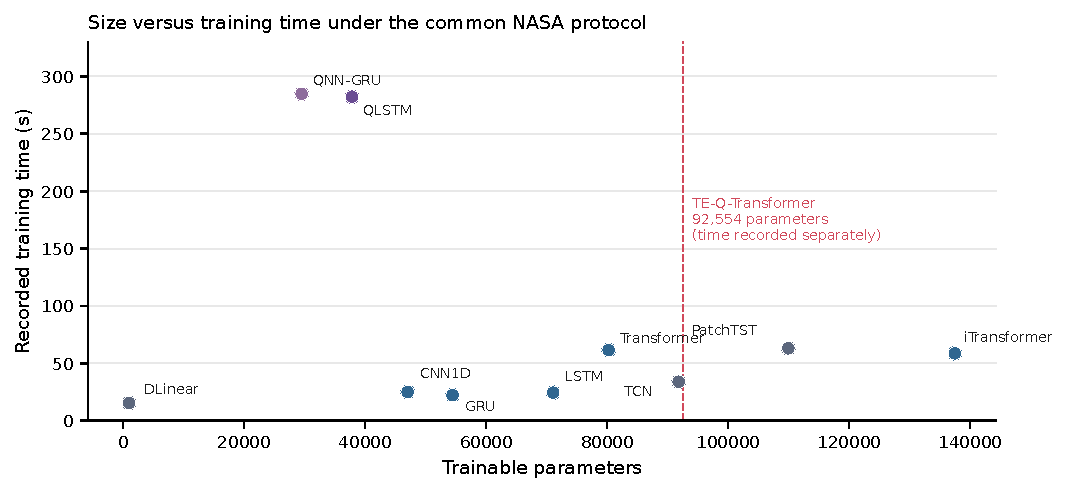
\includegraphics[width=\linewidth]{figs/fig_compute.pdf}
\caption{Trainable parameter count versus recorded training time for the ten models trained from scratch under the common NASA protocol. The dashed line marks the TE-Q-Transformer parameter count. Its training time is recorded separately because the reference configuration was not retrained in that comparison, and later CUDA and CPU-simulator timings are not interchangeable with the common-protocol times.}
\label{fig:compute}
\end{figure}

\subsection{Ablation Study}
\label{sec:ablation}
\label{sec:further_study}

The benchmark ranking does not identify which parts of the proposed design are responsible for the observed behaviour. This section isolates four factors: physics-guided temperature encoding, the SEI and lithium-plating terms, the quantum representation, and architectural components.

\subsubsection{Effect of Physics-Guided Temperature Encoding}
\label{sec:physics_analysis}

To isolate the effect of the temperature representation, the physics-guided encoding was compared with conventional temperature normalization under an otherwise unchanged model (Figure~\ref{fig:physics_contribution}(a); Table~\ref{tab:physics}). Physics-guided encoding lowers macro RMSE from $0.0201$ to $0.0168$, a $16.5\%$ relative reduction. The cell pattern is mixed. RMSE increases on unseen B0018 ($-17.5\%$) and decreases on B0032 ($+34.8\%$) and B0053-test ($+40.4\%$). The B0018 deterioration is retained in Figure~\ref{fig:physics_contribution}(a). The macro gain is therefore not a uniform cell-wise gain.

\subsubsection{Contribution of Temperature-Dependent Mechanisms}
\label{sec:mechanism_analysis}

The individual and combined temperature-dependent mechanisms were then evaluated through an ablation of the SEI term, the lithium-plating term, and both terms together (Figure~\ref{fig:physics_contribution}(b); Table~\ref{tab:physics}). Combined SEI + plating has the lowest macro RMSE in this comparison ($0.0215$), versus plating-only $0.0249$ and SEI-only $0.0330$. Combined encoding is best on B0018 and B0032, but plating-only is best on B0053-test (RMSE $0.0171$ versus combined $0.0222$). The combined representation is therefore the strongest aggregate choice in this study, not a uniformly best choice on every cell.

The physics-guided encoding result in Section~\ref{sec:physics_analysis} and the combined-mechanism result in this subsection come from separate trainings and are not averaged. Learned activation-energy parameters (Table~\ref{tab:ea}) are optimized model scalars, initialized at $3.0$ on the implementation scale. They are not independently measured physical constants. Multi-seed statistics for these parameters were not recorded.

\begin{table*}[htbp]
\centering
\footnotesize
\caption{Physics-guided temperature ablation on the NASA macro split. The encoding comparison and the mechanism comparison are separate trainings.}\label{tab:physics}
\begin{tabular*}{\textwidth}{@{}LCCCC@{}}
\toprule
Variant & RMSE & MAE & MAPE & $R^2$ \\
\midrule
Conventional temperature & 0.0201 & 0.0171 & 1.84 & 0.723 \\
Physics-guided temperature & 0.0168 & 0.0141 & 1.56 & 0.870 \\
SEI-only & 0.0330 & 0.0282 & 2.88 & 0.068 \\
Li-plating-only & 0.0249 & 0.0208 & 2.21 & 0.592 \\
SEI + Li-plating & 0.0215 & 0.0172 & 1.81 & 0.610 \\
\bottomrule
\end{tabular*}
\end{table*}

\begin{table*}[htbp]
\centering
\footnotesize
\caption{Learned activation-energy parameters (seed 42). These are trainable model scalars, not measured physical constants.}\label{tab:ea}
\begin{tabular*}{\textwidth}{@{}LCCC@{}}
\toprule
Variant & Initialization & $E_{a,\mathrm{sei}}$ & $E_{a,\mathrm{pl}}$ \\
\midrule
SEI-only & 3.0 & 2.618 & --- \\
Li-plating-only & 3.0 & --- & 2.180 \\
SEI + Li-plating & 3.0 & 1.981 & 2.820 \\
\bottomrule
\end{tabular*}
\end{table*}

\begin{figure*}[htbp]
\centering
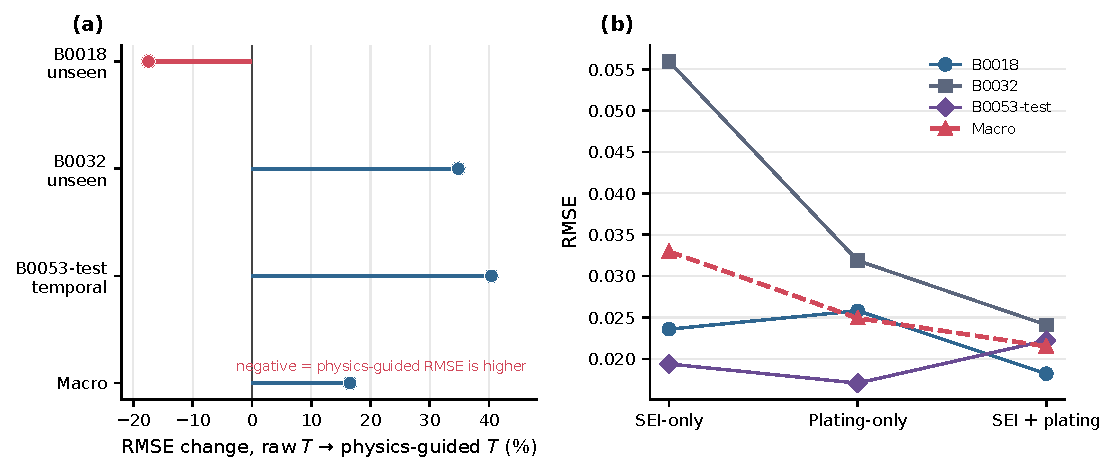
\includegraphics[width=\textwidth]{figs/fig7_physics_contribution.pdf}
\caption{Physics-guided temperature ablation on NASA. (a)~Percent RMSE change from conventional temperature to physics-guided temperature; the B0018 marker is negative. (b)~RMSE from SEI-only to plating-only to combined SEI + Li-plating. Learned $E_a$ values are listed in Table~\ref{tab:ea}.}
\label{fig:physics_contribution}
\end{figure*}

\subsubsection{Contribution of the Quantum Representation}
\label{sec:quantum_analysis}

The contribution of the quantum representation was examined by replacing the four-qubit embedding with a capacity-matched classical representation while keeping the physics-guided temperature encoding (Table~\ref{tab:e04}; Figure~\ref{fig:quantum_contribution}). Quantum + physics records macro RMSE $0.0215$ and $R^2$ $0.610$. Classical + physics records $0.0431$ and $R^2$ $-0.746$. The quantum variant is better on all three NASA settings, including B0018. Parameter counts are nearly matched ($92\,554$ versus $92\,695$). Training on the CPU simulator is slower for the quantum model ($3599$\,s versus $2180$\,s).

The results provide evidence that the tested quantum representation contributes predictive information under the matched experimental setting. They do not establish hardware speedup or a general quantum computational advantage.

\begin{table*}[htbp]
\centering
\footnotesize
\caption{Matched classical versus quantum representation on the NASA macro split. MaxE is the maximum of the three cell-wise maxima. Training times are CPU PennyLane \mbox{\texttt{default.qubit}} simulation.}\label{tab:e04}
\begin{tabular*}{\textwidth}{@{}LCCCCCCC@{}}
\toprule
Variant & RMSE~$\downarrow$ & MAE~$\downarrow$ & MAPE~$\downarrow$ & $R^2$~$\uparrow$ & MaxE~$\downarrow$ & Params & Train (s) \\
\midrule
Classical + physics & 0.0431 & 0.0377 & 3.99 & $-$0.746 & 0.0912 & 92\,695 & 2179.9 \\
Quantum + physics & 0.0215 & 0.0172 & 1.81 & 0.610 & 0.0784 & 92\,554 & 3599.3 \\
\bottomrule
\end{tabular*}
\end{table*}

\begin{figure}[htbp]
\centering
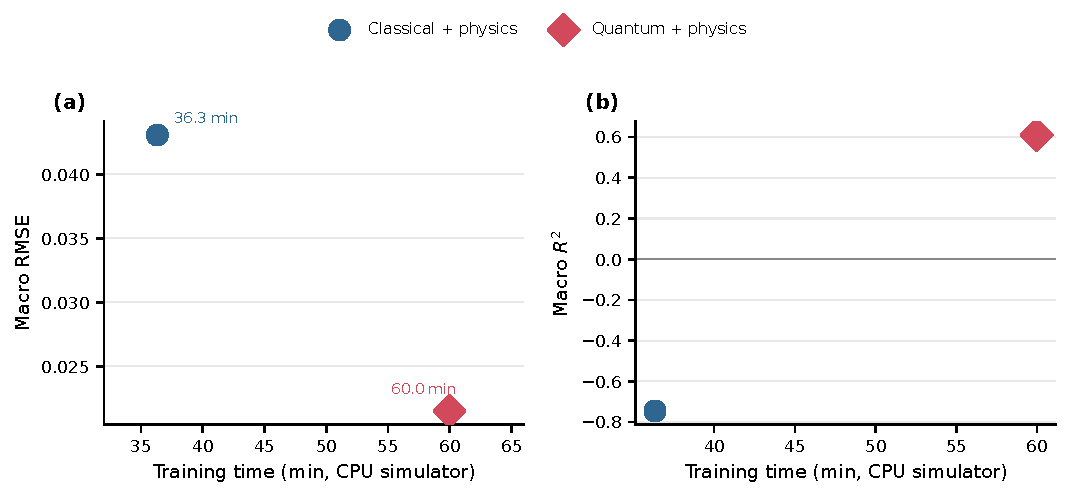
\includegraphics[width=\linewidth]{figs/fig8_quantum_contribution.pdf}
\caption{Matched classical versus quantum representation on the CPU PennyLane simulator. (a)~macro RMSE versus training time; (b)~macro $R^2$ versus training time. Times are simulated execution cost, not hardware quantum runtime.}
\label{fig:quantum_contribution}
\end{figure}

\subsubsection{Architectural Component Analysis}
\label{sec:arch_ablation}

Table~\ref{tab:s1_arch} and Figure~\ref{fig:arch_ablation} report component replacements inside the proposed architecture. Removing or replacing the rich entangler, positional encoding, temporal convolution, CLS pooling, or related blocks increases macro RMSE relative to the full model. The largest degradation is the basic entangler ($+0.0221$ RMSE). A Pauli feature map is the smallest change among the tested variants ($+0.0038$). No tested variant improves on the full model.

These replacements are diagnostic of the proposed architecture. They are not a second ranking of contemporary baselines. MaxE in Table~\ref{tab:s1_arch} follows the original component-ablation convention and should not be compared with the true-cycle maximum of $0.1022$ in Table~\ref{tab:e01_ref}.

\begin{table*}[htbp]
\centering
\footnotesize
\caption{Architectural component ablation on the NASA macro split. $\Delta$RMSE is relative to the full model. MaxE in this table follows the original component-ablation convention and is not the true-cycle maximum reported in Table~\ref{tab:e01_ref}.}\label{tab:s1_arch}\label{tab:nasa_ablation}
\begin{tabular*}{\textwidth}{@{}LLCCCCCC@{}}
\toprule
Settings & Configuration & RMSE & MAE & MAPE & $R^2$ & MaxE & $\Delta$RMSE \\
\midrule
Basic entangler & Rich $\rightarrow$ basic & 0.0388 & 0.0320 & 3.53 & 0.342 & 0.0743 & $+0.0221$ \\
Pauli feature map & $+$ Pauli map & 0.0206 & 0.0166 & 1.78 & 0.774 & 0.0603 & $+0.0038$ \\
No temporal conv. & $-$ temporal conv. & 0.0261 & 0.0231 & 2.50 & 0.618 & 0.0554 & $+0.0093$ \\
GRU smoother & GRU replaces conv. & 0.0274 & 0.0217 & 2.38 & 0.649 & 0.0610 & $+0.0107$ \\
No PE & $-$ positional encoding & 0.0330 & 0.0268 & 2.87 & 0.174 & 0.0862 & $+0.0162$ \\
Mean pooling & Mean pool, no CLS & 0.0237 & 0.0190 & 2.02 & 0.565 & 0.0642 & $+0.0069$ \\
Residual MLP & $+$ residual MLP & 0.0255 & 0.0214 & 2.29 & 0.545 & 0.0628 & $+0.0087$ \\
Full model & Rich, PE, conv $k{=}3$, CLS & 0.0168 & 0.0141 & 1.56 & 0.870 & 0.0493 & --- \\
\bottomrule
\end{tabular*}
\end{table*}

\begin{figure}[htbp]
\centering
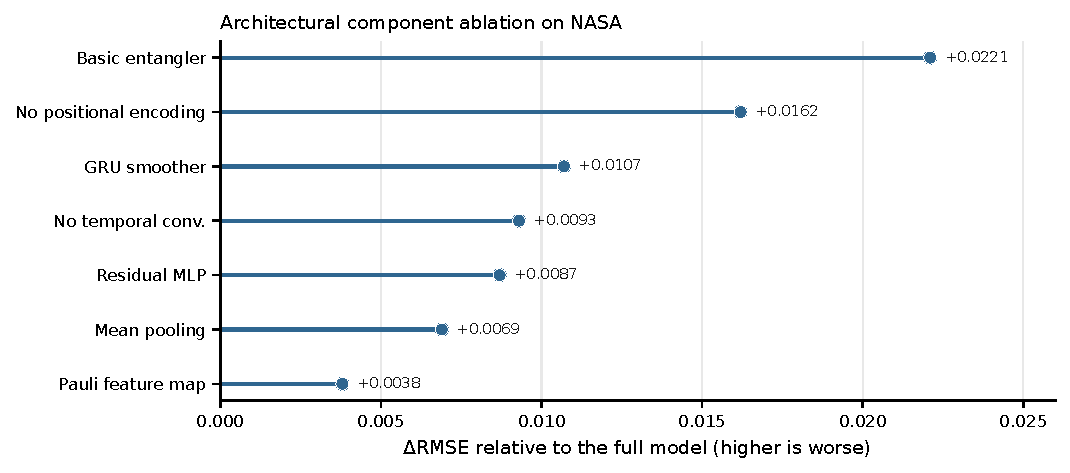
\includegraphics[width=\linewidth]{figs/fig_arch_ablation.pdf}
\caption{Increase in NASA macro RMSE when individual architectural components of TE-Q-Transformer are removed or replaced. Larger values indicate greater degradation relative to the full model.}
\label{fig:arch_ablation}
\end{figure}

\subsection{Generalization and Robustness}
\label{sec:generalization}

The ablation results concern a single validated configuration. The next question is whether useful NASA behaviour remains after independent retraining and across random seeds.

\subsubsection{Cross-Cell and Temporal Generalization}
\label{sec:generalization_analysis}

An independent retraining was used to examine cross-cell and temporal generalization for five models: TE-Q-Transformer, QNN-GRU, iTransformer, Transformer, and PatchTST (Figure~\ref{fig:nasa_generalization}(b)--(d); Table~\ref{tab:e06_cells}). The independently retrained TE-Q-Transformer produced a macro RMSE of $0.02387$, which differs from the validated reference configuration ($0.0168$). The two experiments were conducted under different training configurations, including different weight decay. The two results are therefore retained for their respective evaluation purposes rather than merged.

TE-Q-Transformer is not uniformly best on every metric for every cell. It is strongest on unseen B0018 in this five-model comparison (RMSE $0.0276$, $R^2$ $0.890$). On unseen B0032, PatchTST and iTransformer have lower MAE ($0.0171$ and $0.0185$ versus $0.0189$). On the short B0053 tail, several models remain close, and $R^2$ is modest for all of them. The unseen-cell mean RMSE for TE-Q-Transformer is $0.0240$ with a two-cell range of $0.0072$. QNN-GRU has a slightly smaller RMSE range ($0.0068$) at a higher mean ($0.0369$). These two-cell summaries describe observed variability only.

Figure~\ref{fig:nasa_generalization} shows the corresponding SOH trajectories, including the B0053 train/test boundary. The trajectories belong to the independently retrained models, not to the validated reference in Table~\ref{tab:e01_ref}.

\begin{table*}[htbp]
\centering
\footnotesize
\caption{Independent five-model evaluation of NASA cross-cell and temporal generalization. B0018 and B0032 are unseen cells; B0053-test is temporal extrapolation. TE-Q-Transformer in this table is the independently retrained configuration, not the validated reference in Table~\ref{tab:e01_ref}.}\label{tab:e06_cells}
\begin{tabular*}{\textwidth}{@{}LCCCCCCCCC@{}}
\toprule
 & \multicolumn{3}{c}{B0018 (unseen)} & \multicolumn{3}{c}{B0032 (unseen)} & \multicolumn{3}{c}{B0053-test (temporal)} \\
\cmidrule(lr){2-4}\cmidrule(lr){5-7}\cmidrule(lr){8-10}
Model & RMSE & MAE & $R^2$ & RMSE & MAE & $R^2$ & RMSE & MAE & $R^2$ \\
\midrule
TE-Q-Transformer & 0.0276 & 0.0215 & 0.890 & 0.0204 & 0.0189 & 0.713 & 0.0237 & 0.0209 & 0.184 \\
QNN-GRU & 0.0404 & 0.0344 & 0.765 & 0.0335 & 0.0248 & 0.221 & 0.0286 & 0.0241 & $-$0.195 \\
iTransformer & 0.0691 & 0.0624 & 0.311 & 0.0236 & 0.0185 & 0.613 & 0.0241 & 0.0214 & 0.154 \\
Transformer & 0.0604 & 0.0539 & 0.472 & 0.0335 & 0.0283 & 0.223 & 0.0358 & 0.0303 & $-$0.870 \\
PatchTST & 0.1249 & 0.1061 & $-$1.253 & 0.0222 & 0.0171 & 0.660 & 0.0449 & 0.0410 & $-$1.937 \\
\bottomrule
\end{tabular*}
\end{table*}

\begin{figure*}[htbp]
\centering
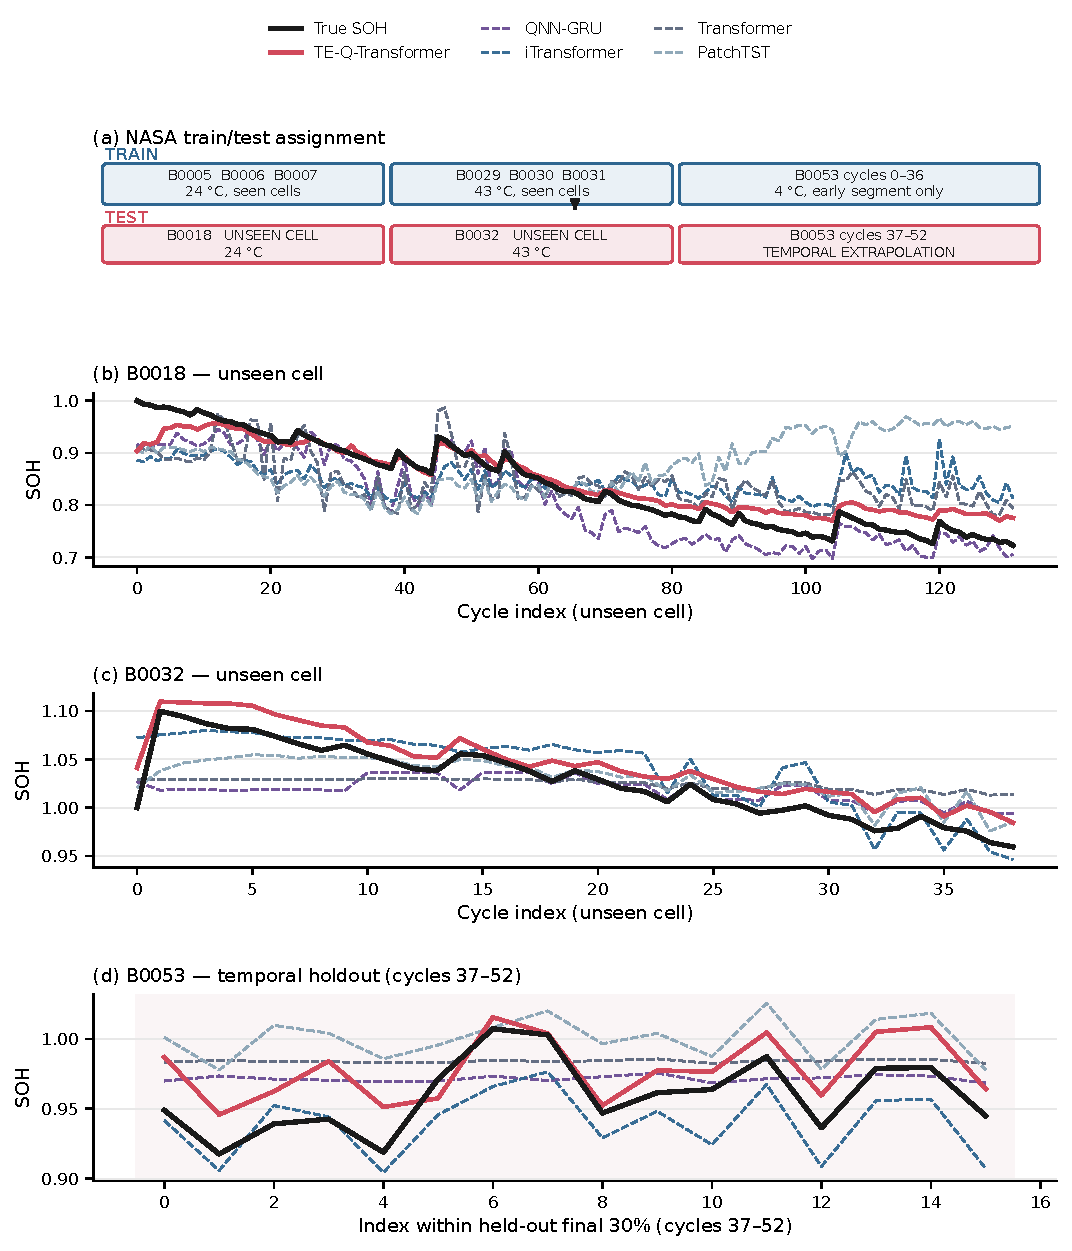
\includegraphics[width=\textwidth]{figs/fig9_nasa_generalization.pdf}
\caption{NASA evaluation protocol and independently retrained SOH trajectories. (a)~Train/test assignment; B0018 and B0032 are unseen cells, and B0053 cycles 37--52 are temporal extrapolation. (b)--(d)~True SOH and five independently retrained models. The TE-Q-Transformer curves are not the validated reference in Table~\ref{tab:e01_ref}.}
\label{fig:nasa_generalization}
\end{figure*}

\subsubsection{Multi-Seed Robustness}
\label{sec:multiseed_analysis}

Five fixed random seeds (42, 43, 44, 45, and 46) were used to evaluate run-to-run variability for the same five models (Figure~\ref{fig:multiseed}; Table~\ref{tab:e07}). TE-Q-Transformer has the lowest mean RMSE ($0.0244\pm0.0096$) but a large coefficient of variation ($0.394$). Seed 43 is an adverse run (overall RMSE $0.0405$, B0032 $R^2=-2.13$). Seed 44 is the best TE-Q run (RMSE $0.0150$). QNN-GRU is more stable (RMSE $0.0381\pm0.0039$) at a higher mean error. Five predefined seeds do not constitute a statistical significance test, and the observed spread does not support a claim of uniform robustness. Figure~\ref{fig:multiseed}(a) identifies each seed; the adverse TE-Q point is retained.

\begin{table*}[htbp]
\centering
\footnotesize
\caption{Run-to-run variability over five predefined seeds (42--46). Values are mean $\pm$ sample standard deviation ($n=5$). This is descriptive evidence only, not a significance test.}\label{tab:e07}
\begin{tabular*}{\textwidth}{@{}LCCC@{}}
\toprule
Model & RMSE & MAE & $R^2$ \\
\midrule
TE-Q-Transformer & $0.0244\pm0.0096$ & $0.0197\pm0.0084$ & $0.455\pm0.534$ \\
QNN-GRU & $0.0381\pm0.0039$ & $0.0328\pm0.0040$ & $-0.432\pm0.467$ \\
iTransformer & $0.0379\pm0.0112$ & $0.0327\pm0.0103$ & $0.133\pm0.733$ \\
Transformer & $0.0367\pm0.0071$ & $0.0312\pm0.0063$ & $0.167\pm0.298$ \\
PatchTST & $0.0466\pm0.0150$ & $0.0389\pm0.0126$ & $0.125\pm0.520$ \\
\bottomrule
\end{tabular*}
\end{table*}

\begin{figure}[htbp]
\centering
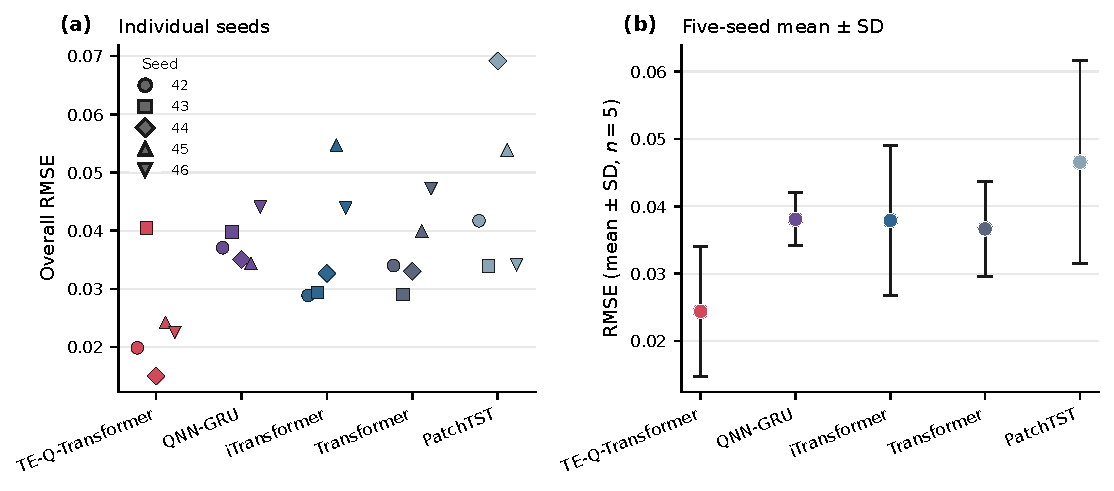
\includegraphics[width=\linewidth]{figs/fig11_multiseed_robustness.pdf}
\caption{Run-to-run variability on five predefined seeds (42--46). (a)~individual overall RMSE by seed; (b)~mean $\pm$ sample standard deviation. The spread is observed variability, not a significance test. The adverse TE-Q-Transformer seed remains visible.}
\label{fig:multiseed}
\end{figure}

\subsection{External Validation on the CALCE Battery Dataset}
\label{sec:calce}

The NASA results above are in-dataset. The remaining question is whether the NASA-trained model transfers, without adaptation, to a different laboratory, cell format, and cycling protocol.

\subsubsection{Dataset Description}
\label{sec:calce_description}

CALCE CS2 cells from the University of Maryland~\citep{w9rg-7173-25} provide a second laboratory and chemistry. The CS2 series are prismatic lithium cobalt oxide cells (nominal $1.1$\,Ah) cycled with CCCV charge and $1$C discharge. Official logs have no thermocouple column, so temperature is filled at a constant $23\,^\circ$C ambient. The external test uses CS2\_35 ($n=880$), CS2\_36 ($n=968$), CS2\_37 ($n=1036$), and CS2\_38 ($n=1025$). Because ambient temperature is fixed by construction, this experiment is not a temperature-generalization test.

\subsubsection{Zero-Shot Cross-Dataset Protocol}
\label{sec:calce_protocol}

The CALCE experiment is zero-shot transfer of the NASA-trained TE-Q-Transformer and the frozen NASA train-only scaler. All four CS2 cells are unseen external test cells. No CALCE training, no CALCE validation, no CALCE model selection, and no CALCE calibration are used. This protocol is stricter than a CALCE-trained cross-cell split.

\subsubsection{External Validation Results and Limitations}
\label{sec:calce_results}

Table~\ref{tab:calce} and Figure~\ref{fig:calce_validation} report a negative-transfer result. Pooled RMSE is $0.3325$, MAE $0.2676$, and $R^2$ $-1.789$ on $3909$ windows. Predictions remain near $1.0$ (archived range approximately $0.978$--$1.041$) while true SOH declines to about $0.14$. A constant predictor of $1.0$ has pooled RMSE $0.3277$, slightly lower than the NASA-trained model. Per-cycle prediction arrays were not retained, so Figure~\ref{fig:calce_validation} shows true and predicted SOH ranges and mean bias rather than reconstructed trajectories.

The result is evidence of limited zero-shot cross-dataset transfer. Strong in-dataset performance on NASA does not automatically imply transfer across a different dataset, laboratory, cell format, and cycling protocol. It is not a failure of the NASA benchmark itself, and it is not a temperature experiment.

\begin{table*}[htbp]
\centering
\footnotesize
\caption{Zero-shot NASA$\rightarrow$CALCE external validation of the NASA-trained TE-Q-Transformer. The NASA scaler is frozen. No CALCE training, validation, or calibration is used.}\label{tab:calce}
\begin{tabular*}{\textwidth}{@{}LCCCC@{}}
\toprule
Cell & $n$ & RMSE~$\downarrow$ & MAE~$\downarrow$ & $R^2$~$\uparrow$ \\
\midrule
CS2\_35 & 880 & 0.2933 & 0.2415 & $-$2.070 \\
CS2\_36 & 968 & 0.3731 & 0.2937 & $-$1.567 \\
CS2\_37 & 1036 & 0.3483 & 0.2803 & $-$1.776 \\
CS2\_38 & 1025 & 0.3061 & 0.2524 & $-$2.115 \\
Pooled & 3909 & 0.3325 & 0.2676 & $-$1.789 \\
\bottomrule
\end{tabular*}
\end{table*}

\begin{figure}[htbp]
\centering
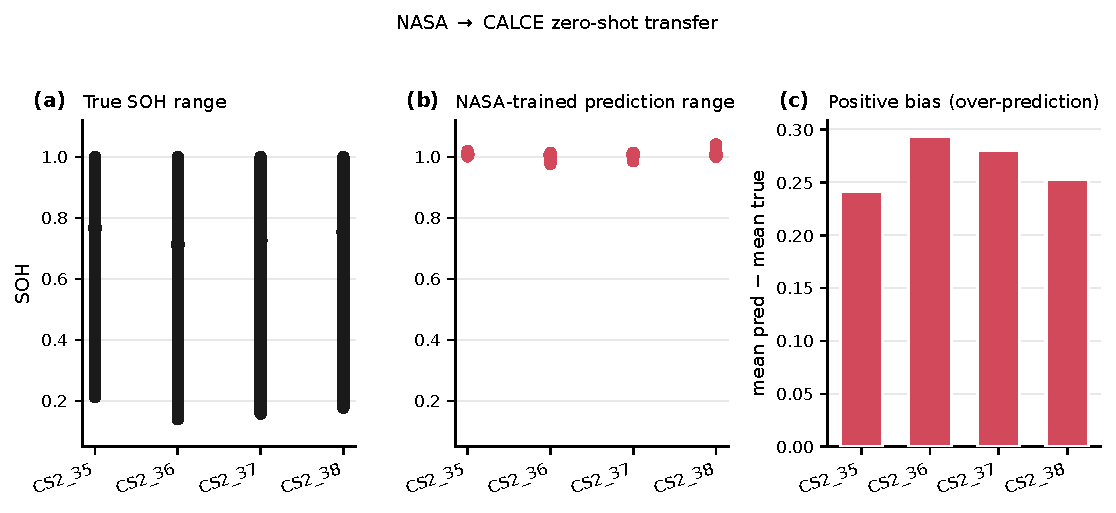
\includegraphics[width=\linewidth]{figs/fig12_calce_validation.pdf}
\caption{Zero-shot NASA$\rightarrow$CALCE transfer of the NASA-trained TE-Q-Transformer. (a)~True SOH range by cell, from the archived minimum to the first-cycle definition of 1.0. (b)~Predicted SOH range. (c)~Mean predicted minus mean true SOH. Per-cycle trajectories were not retained and are not reconstructed.}
\label{fig:calce_validation}
\end{figure}

\clearpage
